\documentclass[9pt]{extarticle}
\title{}
\author{Avinash Iyer}
\date{}

%font setup
%
%\usepackage[math]{anttor}

%paper setup
\usepackage{geometry}
\geometry{letterpaper, portrait, margin=1in}
\usepackage{fancyhdr}

%symbols
\usepackage{amsmath}
\usepackage{amssymb}
\usepackage{hyperref}
\usepackage{gensymb}

\usepackage[T1]{fontenc}
\usepackage[utf8]{inputenc}

%chemistry stuff
\usepackage[version=4]{mhchem}
\usepackage{chemfig}

%plotting
\usepackage{pgfplots}
\usepackage{tikz}

%\usepackage{natbib}

%graphics stuff
\usepackage{graphicx}
\graphicspath{ {./images/} }

%a useful command
\newcommand{\plain}[1]{\textrm{#1}}

%code stuff
%when using minted, make sure to add the -shell-escape flag
%you can use lstlisting if you don't want to use minted
%\usepackage{minted}
%\usemintedstyle{pastie}
%\newminted[javacode]{java}{frame=lines,framesep=2mm,linenos=true,fontsize=\footnotesize,tabsize=3,autogobble,}
%\newminted[cppcode]{cpp}{frame=lines,framesep=2mm,linenos=true,fontsize=\footnotesize,tabsize=3,autogobble,}

\usepackage{listings}
\usepackage{color}
\definecolor{dkgreen}{rgb}{0,0.6,0}
\definecolor{gray}{rgb}{0.5,0.5,0.5}
\definecolor{mauve}{rgb}{0.58,0,0.82}

\lstset{frame=tb,
	language=Java,
	aboveskip=3mm,
	belowskip=3mm,
	showstringspaces=false,
	columns=flexible,
	basicstyle={\small\ttfamily},
	numbers=none,
	numberstyle=\tiny\color{gray},
	keywordstyle=\color{blue},
	commentstyle=\color{dkgreen},
	stringstyle=\color{mauve},
	breaklines=true,
	breakatwhitespace=true,
	tabsize=3
}
\pagestyle{fancy}
\fancyhf{}
\rhead{Avinash Iyer, Tobias Searcy-Jorgensen}
\lhead{Lab 8: Moment of Inertia}
\begin{document}{
\section*{Abstract}
In this laboratory, we performed two experiments with a turntable to determine the linear acceleration of a hanging mass and the moment of inertia.\\
\\
The first experiment dealt with finding linear acceleration. In the first part, we had a turntable that was connected to a hanging mass with a piece of string. When we would let go of the mass, the turntable would start recording the frequency of how fast the turn table is moving and gives us a value every $2$ seconds. We then measured the radius of the striped disk and the radius of the bobbin to get our angular velocity, and from there graphed angular velocity versus time to obtain angular acceleration. Finally, we multiplied angular acceleration by the radius of the bobbin to find the linear acceleration of the falling mass, which we found to be $a = 0.014\pm 0.001$ m/s$^2$. In the second part of the first experiment, we used the turn table again, but instead of using the frequency to measure the velocity, we used a motion sensor placed on the ground that tracked the falling mass itself. After graphing the results of the motion sensor, we performed a linear regression to find the acceleration \textendash which was found to be $0.0136\pm 0.0001$ m/s$^2$. These results were consistent with each other.\\
\\
In the second experiment, we attempted to find the moment of inertia of two cylinders placed at the ends of each arm of the turntable. To do this, we used a formula to find the moment of inertia given the linear acceleration of the falling mass, namely $mr^2(g/a-1)$, where $m$ is the mass of the falling mass, $r$ is the radius of the bobbin, and $a$ is the linear acceleration of the falling mass. Using the data from the first experiment, we calculated $I_{0} = 0.00281\pm 0.00002$ kg$\cdot$m$^2$. Then, the masses were attached to the edges of the turntable arms and a similar set of trials as the first experiment were performed. The trials yielded a value $I_{\plain{total}} = 0.00606\pm 0.00005$ kg$\cdot$m$^2$. Finally, $I_{0}$ was subtracted from this value to yield $I_{\plain{exp}} = 0.00325\pm 0.00005$ kg$\cdot$m$^2$. Using various measurements of the cylinders, theoretical values of $I_{\plain{theo, pt}} = 0.00324\pm 0.000004$ and $I_{\plain{theo, cyl}} = 0.0033\pm 0.0002$ were found by treating the cylinders as point masses and cylinders respectively.\\
\\
Since the experimental and theoretical results for $I$ were consistent with each other, we conclude that our experimental methods were sound.
\section*{Introduction}
The goal of the first experiment was to use reported frequencies on a striped turntable to find angular velocity and angular acceleration with the ultimate goal of finding the linear acceleration of a falling mass that was pulling a bobbin attached to the turntable. We performed the experiment only once, yielding five different frequency measurements; the angular velocity values that resulted from the frequency measurements were plotted on the $y$ axis against $t$ on the $x$ axis, and a linear regression was performed to find the value of angular acceleration. This value of angular acceleration was multiplied by the radius of the bobbin to find $a$. The second part of this experiment used a motion sensor to find the value of $a$ by plotting velocity against time and using a linear regression on the data.\\
\\
The goal of the second experiment was to find the value of moment of inertia of two cylinders attached to the ends of the arms of the turntable, using a similar methodology to the first experiment. We used the frequency measurements to find the angular velocity of the turntable at each point, then found angular acceleration using the \texttt{LINEST} linear regression function, then found linear acceleration similar to how we found the linear acceleration in the first experiment. Afterwards, we used the equation $I = mr^2(g/a-1)$ using the $m$ for the falling mass. The moment of inertia of the two cylinders was found by subtracting the value of the moment of inertia of the turntable without the cylinders from the value of the moment of inertia with the two cylinders.
\section*{Methods}
In the pre-lab, we found that given a falling mass $m$ with linear acceleration $a$, we could find the moment of inertia of a turntable that the mass was pulling by using $I = mr_b^2(g/a-1)$, where $r_b$ is the radius of the bobbin that the mass is pulling. \\
\\
The linear acceleration of the mass is found by $a = r_b\alpha$, where $\alpha$ is the angular acceleration of the turntable and $r$ is the radius of the bobbin that the mass is pulling.\\
\\
The value of $\alpha$ is found by performing a linear regression on the values of $\omega$.\\
\\
The value of $\omega$ is found by multiplying the frequency reported on the turntable by $x = 0.002$ m, the spacing between each stripe, and then dividing by $r_d$, the radius of the large disk on the turntable. In other words, $\omega = f \frac{x}{r}$. The mathematical process was detailed in the pre-lab.\\
\\
All reported frequency measurements were found while the mass had downward velocity. Any frequency measurements made after the mass reached the bottom of its trajectory and had an upward velocity were disregarded. \\
\\
The radius of the bobbin and the large disk were found using Vernier calipers that had up to $0.05$ mm precision. The masses were found using a triple beam balance that had a precision to the nearest $0.0001$ kg. Non-instrumental experimental uncertainties were negligible, and all instrumental uncertainties were minimized through this process.
\begin{center}
	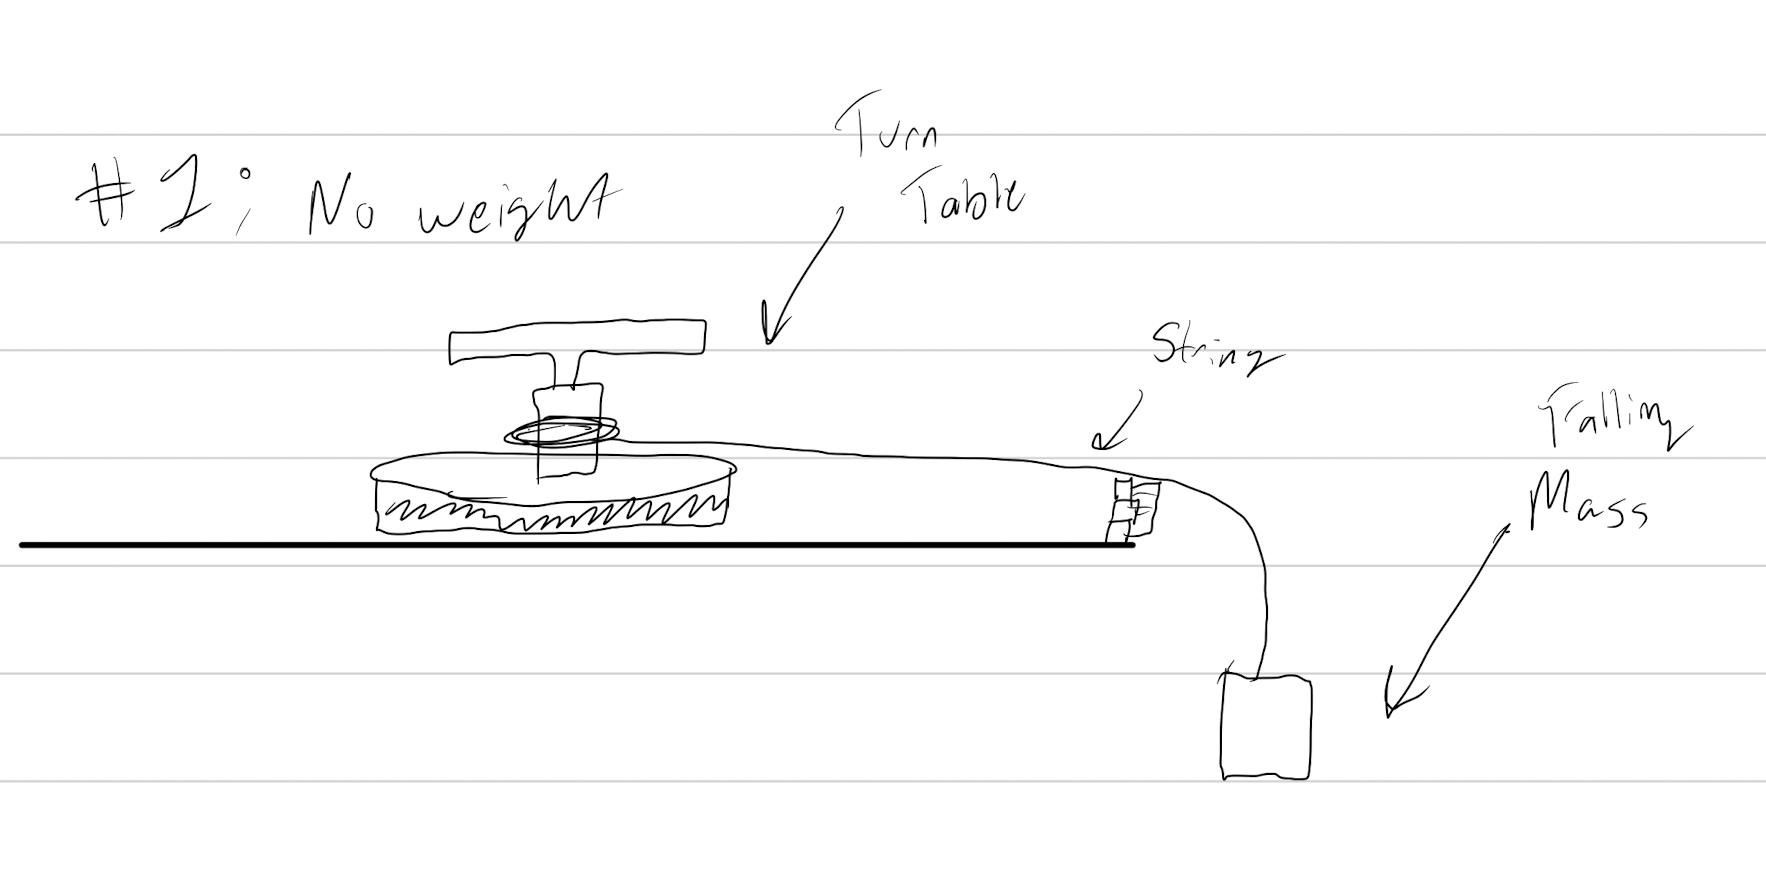
\includegraphics[width=10cm]{images/Lab8Image3_1.png} \\
	Setup for Experiment 1
\end{center}
\begin{center}
	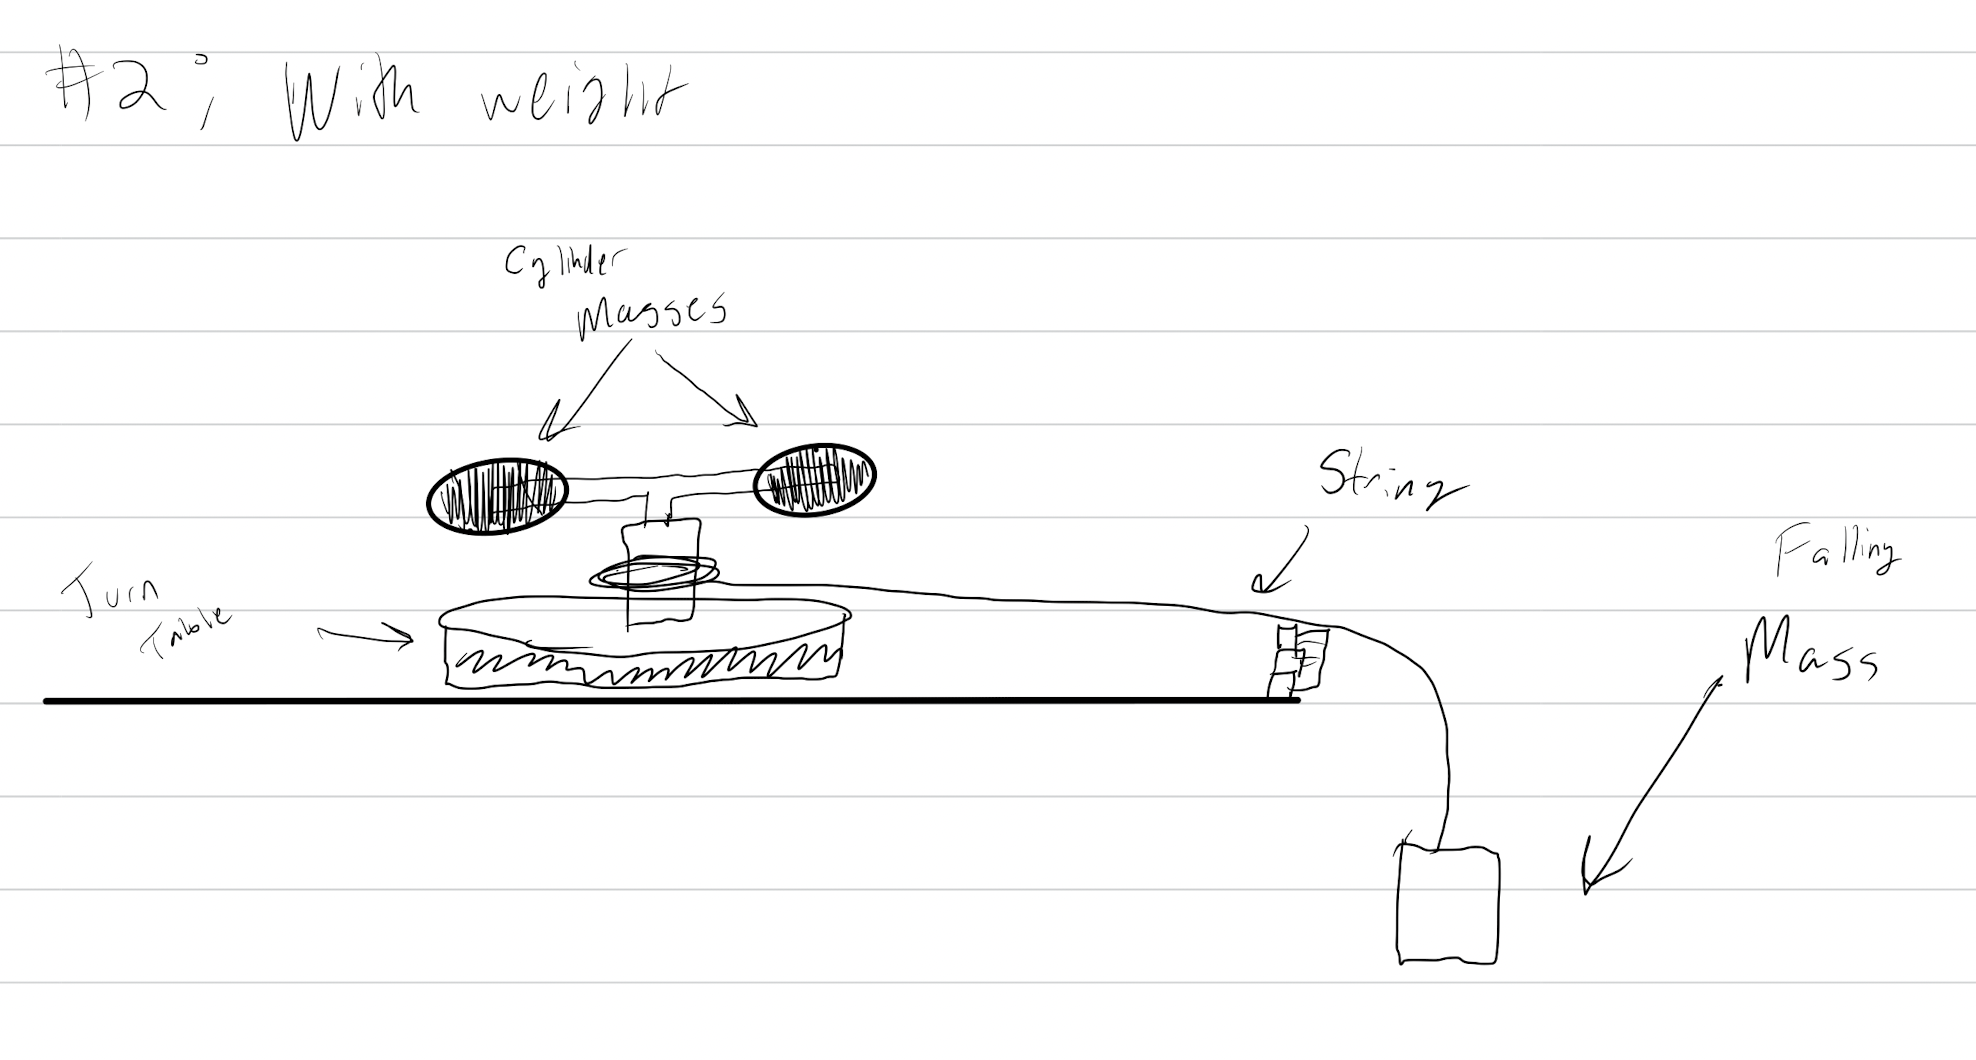
\includegraphics[width=10cm]{Lab8Image3_2.png} \\
	Setup for Experiment 2
\end{center}
\section*{Results and Discussion}
\subsection*{Experiment 1}

\begin{center}
	\renewcommand{\arraystretch}{1.5}
	\begin{tabular}{c|c}
		Value & Measurement \\
		\hline
		Falling mass ($m_3$) & $0.0252\pm 0.0001$ kg\\
		Spacing between Stripes & $0.002$ m \\
		Large Disk Diameter  & $0.12680\pm 0.00005$ m\\
		Large Disk Radius ($r_{d}$)& $0.06340\pm 0.00005$ m \\
		Bobbin Diameter & $0.02500\pm 0.00005$ m \\
		Bobbin Radius ($r_{b})$& $0.01250\pm 0.00005$ m
	\end{tabular}
\end{center}

\begin{center}
	\renewcommand{\arraystretch}{1.5}
	\begin{tabular}{c|c|c}
	 Time (s) & Frequency (hz) & Angular Velocity (s$^{-1}$) \\
	 \hline
	 $2.0\pm 0.1$ & $28$ & $0.88\pm 0.03$\\
	 $4.0\pm 0.1$ & $99$ & $3.12\pm 0.03$\\
	 $6.0\pm 0.1$ & $169$ & $5.33\pm 0.03$\\
	 $8.0\pm 0.1$ & $239$ & $7.53\pm 0.03$\\
	 $10.0\pm 0.1$ & $306$ & $9.65\pm 0.03$
	\end{tabular}
\end{center}

\begin{center}
	\begin{tikzpicture}
		\begin{axis}[
			title={$t$ vs $\omega$, with linear regression},
			xlabel={$t$ (s)},
			ylabel={$\omega$ (s$^{-1}$)},
			xmin=-0.2,xmax=10.2,
			ymin=-0.2,ymax=10,
			xtick={0,2,4,6,8,10},
			ytick={0,2,4,6,8,10},
			xmajorgrids=true,
			ymajorgrids=true,
			grid style=dashed,
			legend pos=south east,
		]
			\addplot[only marks, mark=o, error bars/.cd, y dir = both, x dir = both, x explicit, y explicit]
			table[x index=0, y index=1, y error index=2, x error index=3]{images/Lab8Data1.dat};
			\addlegendentry{\tiny Data}
			\addplot[color=red,thin,domain=0:10,samples=100]{1.10*x-1.28};
			\addlegendentry{\tiny $\omega = 1.10t-1.28$}
		\end{axis}
	\end{tikzpicture}
\end{center}
Performing linear regression on the dataset, we receive the following value for the slope, or angular acceleration:
\[\alpha = 1.10\pm 0.01~\plain{s$^{-2}$}\]
Therefore, the value of linear acceleration is equal to $a = r_{b}\alpha = 0.014\pm 0.001~\plain{m/s$^2$}$.\\
\\
Using the motion sensor, we received the following graph with the value of acceleration of $m = 0.0136\pm 0.0001~\plain{m/s$^2$}$:
\begin{center}
	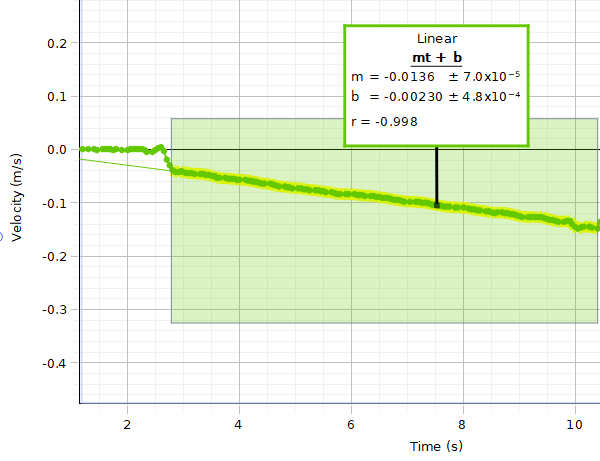
\includegraphics[width=10cm]{Lab8Image4_1}
\end{center}
\subsection*{Discussion}
These values for $a$ are consistent with each other within experimental error. The values were as follows:
\begin{center}
	\renewcommand{\arraystretch}{1.5}
	\begin{tabular}{c|c}
		Value & Measurement \\
		$a_1$ (Stripe Frequency) & $0.014\pm 0.001$ m/s$^2$ \\
		$a_2$ (Motion Sensor) & $0.0136\pm 0.0001$ m/s$^2$
	\end{tabular}
\end{center}
\subsection*{Experiment 2}
\begin{align*}
	I_{0} &= (m_3)(r_b^2)(g/a - 1)\\
	&= 0.00281\\
	\delta I_{0} &= (2)(\delta r_b/r_b)(I_{0}) \\
	&= 0.00002
\end{align*}
To calculate $I_{0}$, we used the largest fractional error, which was of $r_b^2$, or $2(\delta r_b/r_b)$.\\
\begin{center}
	\renewcommand{\arraystretch}{1.5}
	\begin{tabular}{c|c}
		Value & Measurement \\
		\hline
		Cylinder 1 ($m_1$) & $0.2003\pm 0.0001$ kg\\
		Cylinder 2 ($m_2$) & $0.2003\pm 0.0001$ kg \\
		Falling mass ($m_3$) & $0.0252\pm 0.0001$ kg\\
		Spacing between Stripes & $0.002$ m \\
		Large Disk Diameter  & $0.12680\pm 0.00005$ m\\
		Large Disk Radius ($r_{d}$)& $0.06340\pm 0.00005$ m \\
		Bobbin Diameter & $0.02500\pm 0.00005$ m \\
		Bobbin Radius ($r_{b})$& $0.01250\pm 0.00005$ m
	\end{tabular}
\end{center}
\begin{center}
	\renewcommand{\arraystretch}{1.5}
	\begin{tabular}{c|c|c}
	Time (s) & Frequency (hz) & Angular Velocity (s$^{-1}$) \\
	\hline
	2 & $29$ & $0.92$ \\
	4 & $61$ & $1.92$ \\
	6 & $93$ & $2.93$ \\
	8 & $127$ & $4.01$ \\
	10 & $159$ & $5.02$ \\
	12 & $190$ & $5.99$ \\
	14 & $222$ & $7.00$
	\end{tabular}
\end{center}
Using the \texttt{LINEST} function in Google Sheets, we find an equation of $\omega = 0.508t - 0.099$, with a slope of $0.508\pm 0.002$, or an angular acceleration of $\alpha = 0.508\pm 0.002$ s$^{-2}$. Then, we find an acceleration of $a = r_b\alpha$, or $a = 0.00636\pm 0.00003$ m/s$^2$.
\begin{align*}
	I_{\plain{total}} &= (m_3)(r_b^2)(g/a - 1)\\
	&= 0.00606\\
	\delta I_{\plain{total}} &= (2)(\delta r_b/r_b)(I_{\plain{total}})\\
	&= 0.00005
\end{align*}
We used the same technique as calculating $I_{0}$, where we used the maximum fractional uncertainty of $2(\delta r_b/r_b)$. Therefore, the MOI of the masses of the cylinders is $I_{\plain{exp}} = I_{\plain{total}} - I_{0} = 0.00325\pm 0.00005$ kg$\cdot$m$^2$.\\
\\
We will calculate the theoretical values of the moment of inertia by treating the cylinders as point masses with a diameter of $0.180\pm 0.001$ m, with radius $0.090\pm 0.001$m, yielding the following:
\begin{align*}
	I_{\plain{theo, pt}} &= m_{1}r^2 + m_{2}r^2\\
	&= 0.00324\pm 0.00004
\end{align*}
The moment of inertia for a cylinder with thickness is as follows:
\begin{align*}
	I = \frac{1}{12}(m)(r_c^2 + 3l^2)
\end{align*}
Using values of $r_c = 0.0160\pm 0.001$ and $l = 0.033\pm 0.001$, we get a moment of inertia for each cylinder of $I_{1} = 0.000031\pm 0.000002$. Then, using the parallel axis theorem of $I_{2} = I_{1} + mr^2 = 0.0017\pm 0.0001$. Finally, including the fact that there are two cylinders, we get $I_{\plain{theo,cyl}} = 0.0033\pm 0.0002$.
\subsection*{Discussion}
All these results are consistent with each other within the levels of experimental error. We got final values of the following:
\begin{center}
	\renewcommand{\arraystretch}{1.5}
	\begin{tabular}{c|c}
	Value & Measurement \\
	\hline
	$I_{0}$ & $0.00281\pm 0.00002$ kg$\cdot$m$^2$ \\
	$I_{\plain{total}}$ & $0.00606\pm 0.00005$ kg$\cdot$m$^2$\\
	$I_{\plain{exp}}$ & $0.00325\pm 0.00005$ kg$\cdot$m$^2$ \\
	$I_{\plain{theo, pt}}$ & $0.00324\pm 0.00004$ kg$\cdot$m$^2$ \\
	$I_{\plain{theo, cyl}}$ & $0.0033\pm 0.0002$ kg$\cdot$m$^2$
	\end{tabular}
\end{center}
\section*{Conclusion}
The experimental value for the acceleration of the falling mass was consistent with the measured values from the motion sensor. Additionally, the experimental value of the moment of inertia of the two cylinders was consistent with both of the theoretical predictions for the value of the moment of inertia. Even though these results were consistent, in the future we could also account for air resistance, friction, and other errors on the experimental setup.
}\end{document}